\subsection{Impedance Insights: Unlocking the Wonders of 1/8-Wavelength Lines!}

\begin{tcolorbox}[colback=gray!10, colframe=black, title=E9F10] What impedance does a 1/8-wavelength transmission line present to an RF generator when the line is shorted at the far end?

\begin{enumerate}[label=\Alph*.]
    \item A capacitive reactance
    \item The same as the characteristic impedance of the line
    \item \textbf{An inductive reactance}
    \item Zero
\end{enumerate} \end{tcolorbox}

\subsubsection{Related Concepts}

In radio frequency (RF) communications, understanding the behavior of transmission lines is crucial for efficient signal transfer. A 1/8-wavelength transmission line, if terminated in a short circuit at the far end, exhibits particular impedance characteristics that can be analyzed using transmission line theory.

To comprehend this question, we must familiarize ourselves with the following key concepts:

1. \textbf{Transmission Line Basics:}: A transmission line is characterized by its characteristic impedance \( Z_0 \), which is the impedance that the line would present if it were infinitely long. Common types include coaxial cables and microstrip lines.

2. \textbf{Wavelength and Electrical Length:}: The wavelength \( \lambda \) of the signal is determined by the frequency of the RF signal and the velocity of propagation in the line. At a frequency \( f \) and speed of light \( c \), \( \lambda \) is given by:
   \[
   \lambda = \frac{c}{f}
   \]
   A 1/8-wavelength line measures \( \frac{\lambda}{8} \).

3. \textbf{Reflection and Impedance Transformation:}: The impedance seen at the input of a transmission line can be transformed based on its length and the termination at the far end. For a short circuit (zero ohms) terminated at the end of a transmission line:
   - If the line length is a quarter-wavelength (1/4), the impedance at the input becomes the infinite impedance or open circuit.
   - In contrast, at an 1/8-wavelength, the impedance transforms into an inductive reactance.

4. \textbf{Inductive Reactance:}: The inductive reactance \( X_L \) is defined as:
   \[
   X_L = 2 \pi f L
   \]
   where \( L \) is the inductance. For a shorted transmission line, it behaves like a coil (inductance occurs).

Thus, since the 1/8-wavelength line presents an inductive reactance when shorted at the far end, 

\subsubsection{Calculation Example}

To illustrate this, let's analyze a transmission line with a characteristic impedance \( Z_0 \). While we won't delve into complex calculations here, we can assert:

1. The input impedance \( Z_{in} \) at an 1/8 wavelength with a short at the end can qualitatively be stated to be:
\[
Z_{in} = jX_L
\]
which confirms that it acts as an inductance.

2. If needed, specific cases can be calculated if numerical values of \( Z_0 \) and frequency \( f \) are given.

\subsubsection{Diagrammatic Representation}

\begin{center}
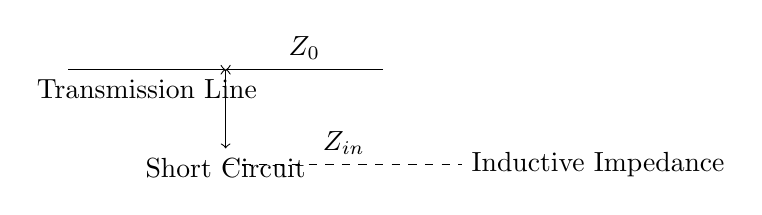
\begin{tikzpicture}
    \draw[->] (0,0) -- (2,0) node[midway, below] {Transmission Line};
    \draw[->] (2,0) -- (2,-1) node[below] {Short Circuit};
    \draw[->] (4,0) -- (2,0) node[pos=0.5, above] {$Z_0$};
    \draw[dashed] (2,-1.2) -- (5,-1.2) node[right] {Inductive Impedance} node[pos=0.5, above] {$Z_{in}$};
\end{tikzpicture}
\end{center}

Therefore, the impedance presented to the RF generator when the line is shorted at the far end is indeed an inductive reactance. This understanding enables radio engineers to design more effective RF systems.
